\documentclass{article}
\usepackage[utf8]{inputenc}
\usepackage[margin=0.5in]{geometry}
\usepackage[portuguese]{babel}
\usepackage{graphicx}
\usepackage{amsmath}
\graphicspath{ {./images/} }

\title{Sinais e Sistemas - Trabalho 1 - Grupo 2}
\author{
    Leonardo Soares da Costa Tanaka \\
    Matheus Henrique Sant Anna Cardoso \\
    Theo Rudra Macedo e Silva
}

\date{Setembro de 2022}

\begin{document}

\maketitle

1.) Para o sinal abaixo, contínuo por partes e definido para $t \in [-5\;5]$: (a) esboçar gráfico, (b) encotrar uma expressão analítica usando sinais singulares, (c) escrever um programa que rode em Octave/MatLab para plotar o gráfico. Nos dados a seguir, as expressões entre vírgulas se referem, na ordem de apresentação, aos valores do sinal nos intervalos $I_{1} = [-5\;-3], I_{2} = [-3\;-1], I_{3} = [-1\;1], I_{4} = [1\;3], I_{5} = [3\;5]$.
\textbf{G2}: $x(t) = -3, 3t + 6, -3t^3, 3t - 6, -t^2 + 5t - 3$

\vspace{\baselineskip}

(a) Esboçando o gráfico:

\begin{figure}[h]
    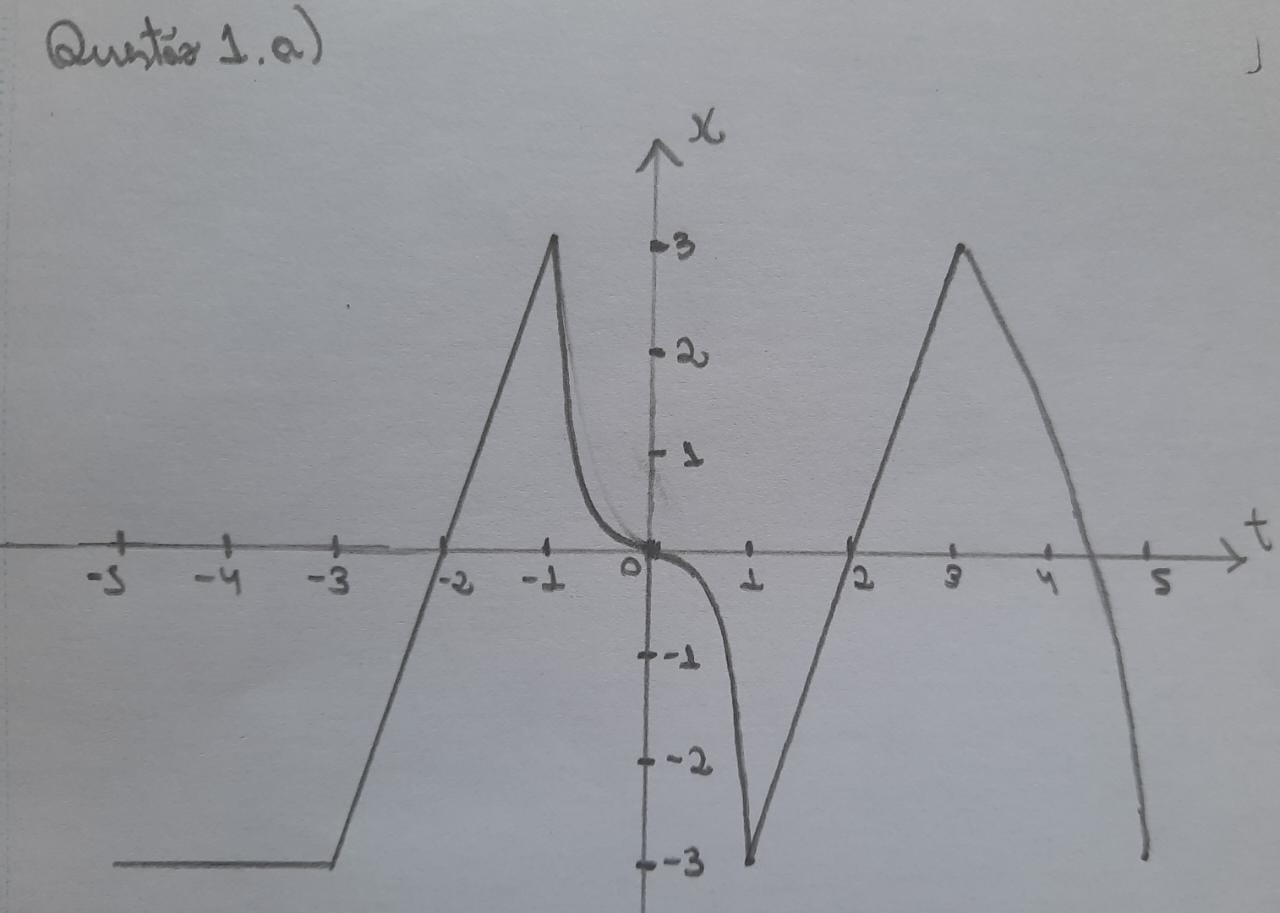
\includegraphics[scale=0.23]{plot1a}
    \centering
\end{figure}

\vspace{\baselineskip}

(b) Analisando para os intervalos, teremos:

\vspace{\baselineskip}

Para $ -5 \leq t < -3, x(t) = -3 $, ou, $ x(t) = -3 \cdot 1(-t) $ utilizando um degrau refletido.

\vspace{\baselineskip}

Para $ -3 \leq t < -1, x(t) = 3t + 6 $, ou, $ x(t) = 3t \cdot 1(-t) + 6 \cdot 1(-t) $ utilizando degrau e rampa unitários.

\vspace{\baselineskip}

Para $ -1 \leq t < 0, x(t) = -3t^3 $, ou, $ x(t) = -6t \cdot \frac{t^2}{2}1(-t) $ utilizando a parábola unitária.

\vspace{\baselineskip}

Para $ 0 \leq t < 1, x(t) = -3t^3 $, ou, $ x(t) = -6t \cdot \frac{t^2}{2}1(t) $ utilizando a parábola unitária.

\vspace{\baselineskip}

Para $ 1 \leq t < 3, x(t) = 3t - 6 $, ou, $ x(t) = 3t \cdot 1(t) - 6 \cdot 1(t) $ utilizando degrau e rampa unitários.

\vspace{\baselineskip}

Para $ 3 \leq t < 5, x(t) = -t^2 + 5t - 3 $, ou, $ x(t) = -2 \cdot \frac{t^2}{2}1(t) + 5t \cdot 1(t) - 3 \cdot 1(t)$ utilizando parábola, rampa e degrau unitários.

\vspace{\baselineskip}

Dessa forma, teremos $x(t)$ definido como:

\[ x(t) = 
\begin{cases} 
    -3 \cdot 1(-t) & -5 \leq t < -3 \\

    3t \cdot 1(-t) + 6 \cdot 1(-t) & -3 \leq t < -1 \\

    -6t \cdot \frac{t^2}{2}1(-t) & -1 \leq t < 0 \\

    -6t \cdot \frac{t^2}{2}1(t) & 0 \leq t < 1 \\

    3t \cdot 1(t) - 6 \cdot 1(t) & 1 \leq t < 3 \\

    -2 \cdot \frac{t^2}{2}1(t) + 5t \cdot 1(t) - 3 \cdot 1(t) & 3 \leq t < 5 
 \end{cases}
\]


\vspace{\baselineskip}

(c) Executando os códigos escritos no arquivo {\tt questao1.m} (feito no Octave), plotamos o seguite gráfico:

\begin{figure}[h]
    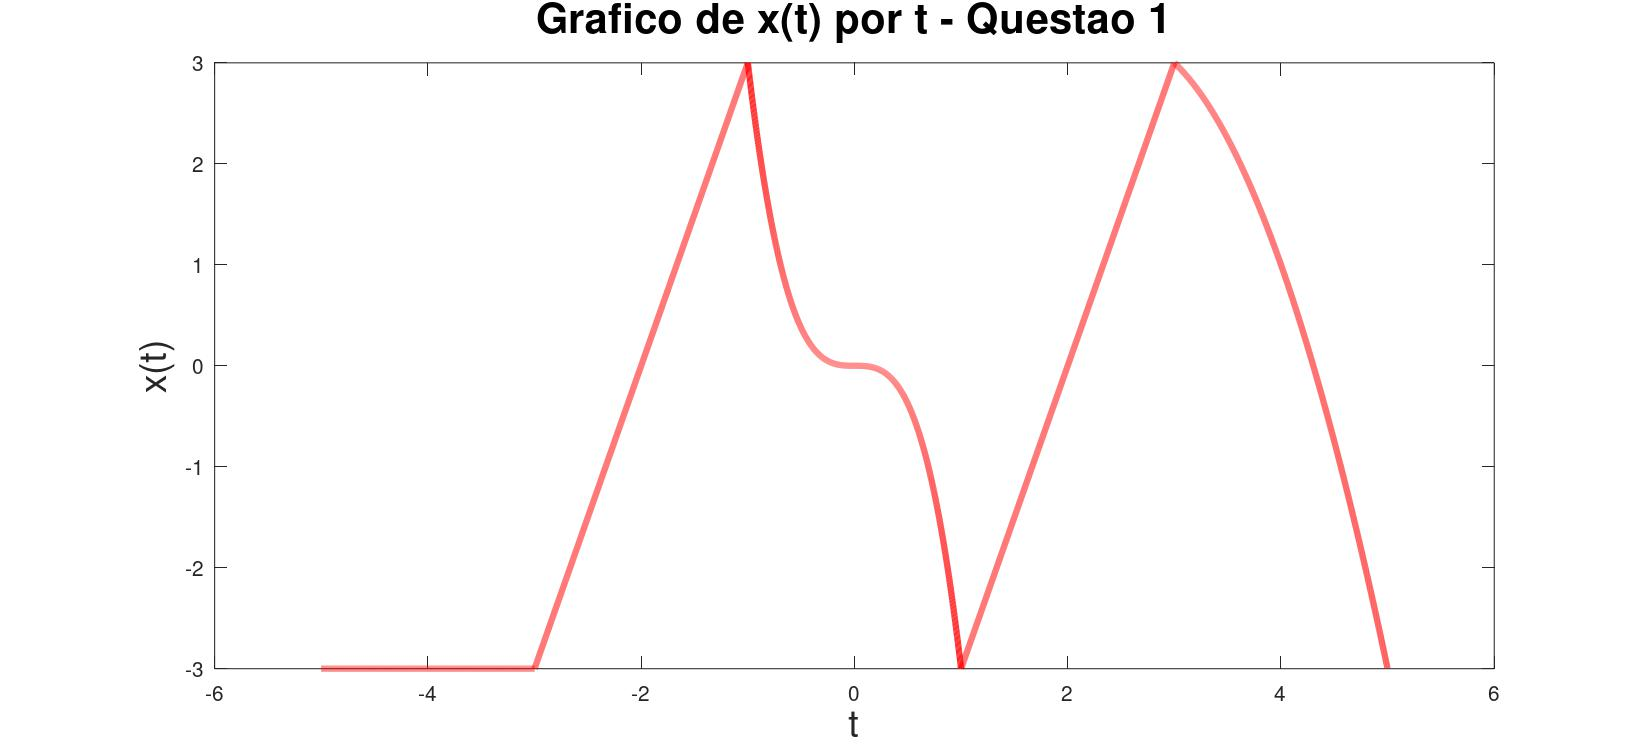
\includegraphics[scale=0.23]{plot1c}
    \centering
\end{figure}

2.) Plotar o gráfico dos sinais a seguir, com escalas adequadas e usando os valores numéricos desejados para os eventuais parâmetros. Dizer se estes sinais são periódicos e, em caso afirmativo quais os seus períodos fundamentais.
(a) $x(t) = sen(\pi t) + cos(2 \pi t) / 2 + sen(3 \pi t) / 3 + cos(4 \pi t) / 4$,
(b) $x(t) = sen(\omega t)cos(50\omega t)$,
(c) $x(t) = sen(\omega t^2)$,
(d) $x(t) = sen(\omega_{1}sen(\omega_{2}t)t)$

\vspace{\baselineskip}

(a) Plotando o gráfico no Octave, temos:

\vspace{\baselineskip}

\begin{figure}[h!]
    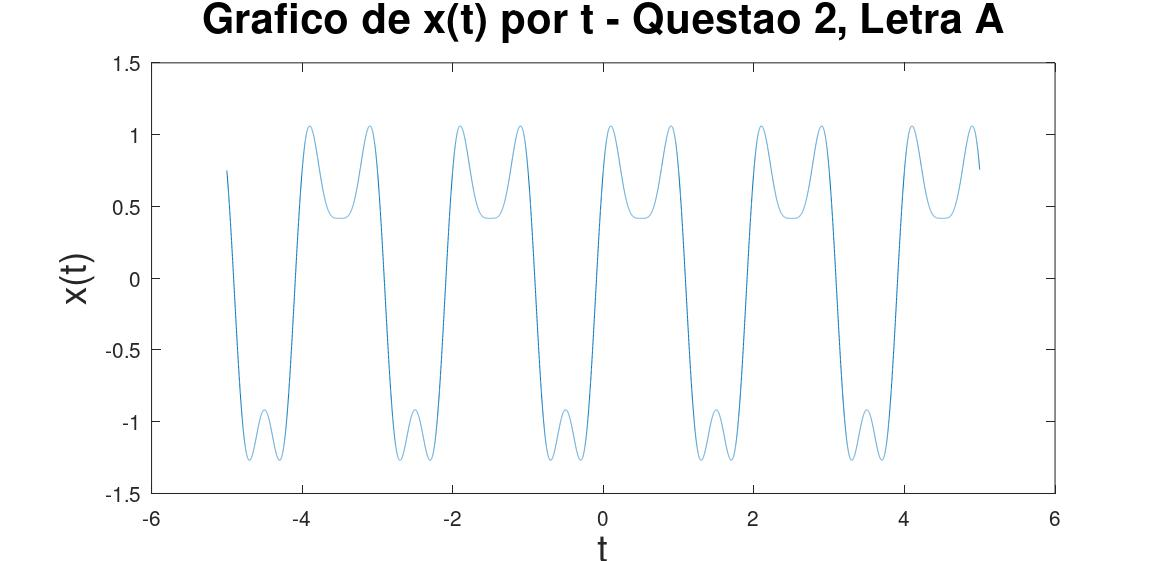
\includegraphics[scale=0.3]{plot2a}
    \centering
\end{figure}

\newpage

(b) Plotando o gráfico no Octave, temos:

\vspace{\baselineskip}

\begin{figure}[h!]
    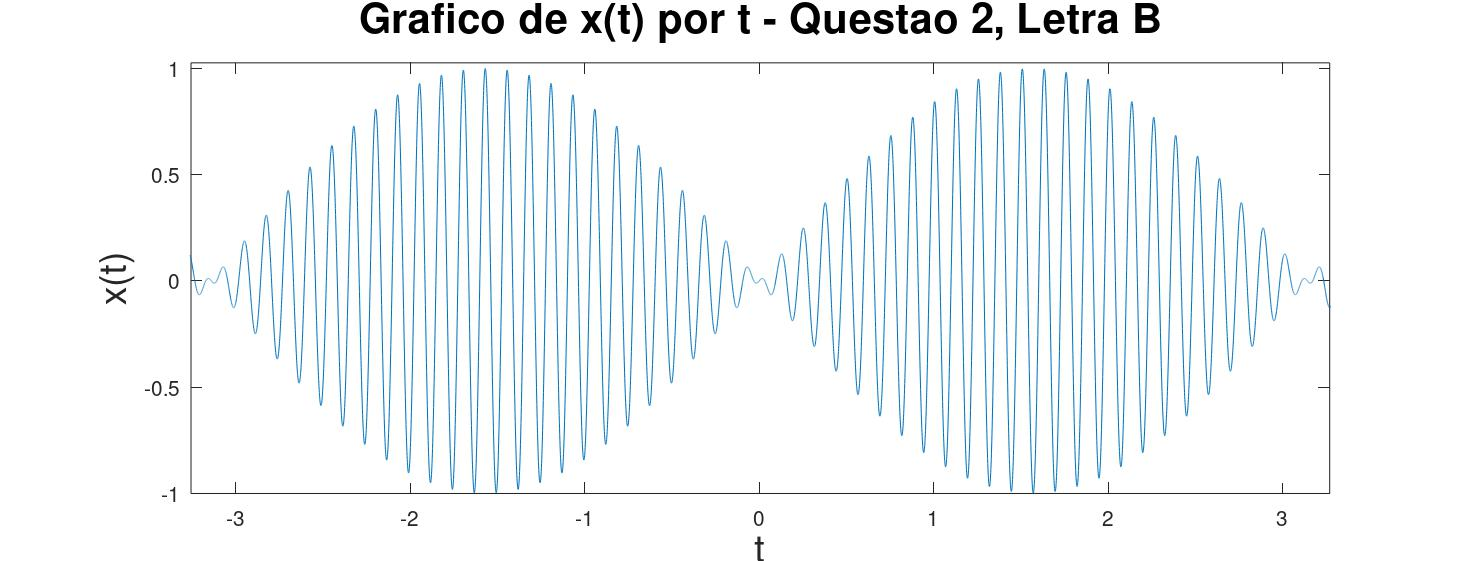
\includegraphics[scale=0.3]{plot2b}
    \centering
\end{figure}

\vspace{\baselineskip}

(c) Plotando o gráfico com o Octave para $\omega = 7$, temos:
\begin{figure}[h!]
    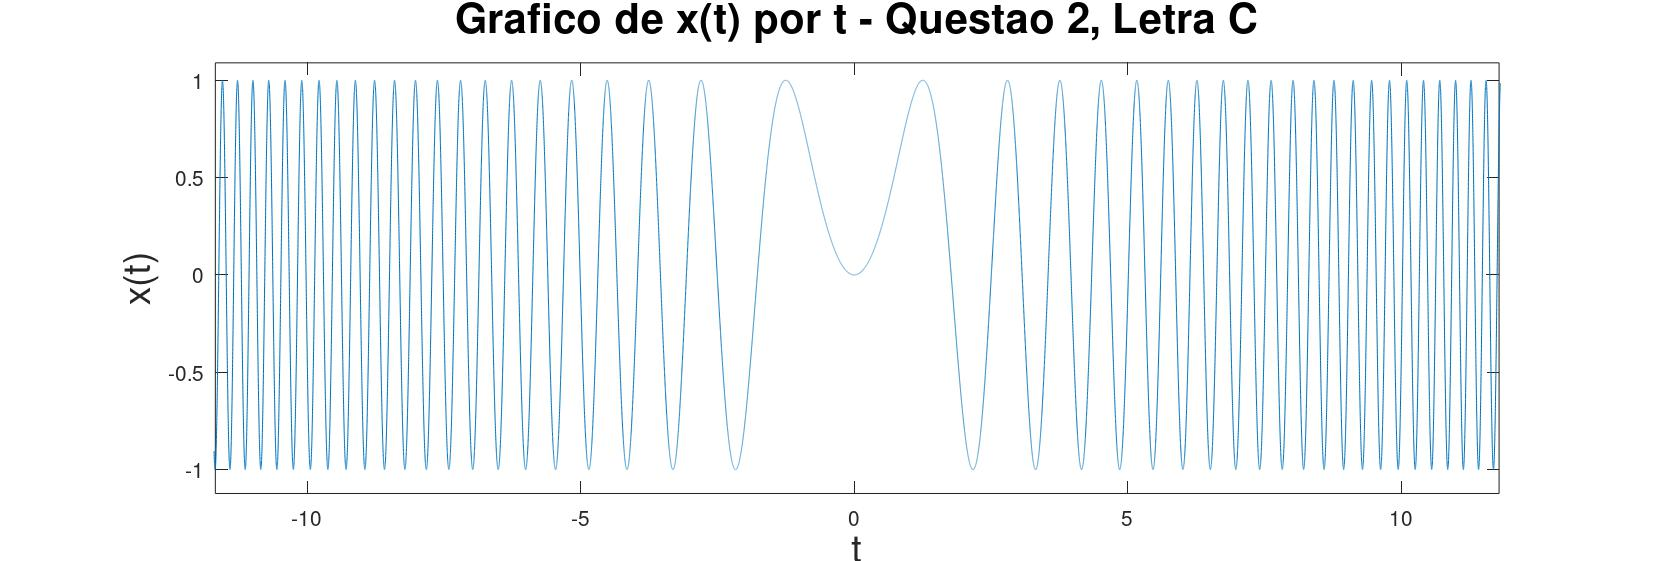
\includegraphics[scale=0.3]{plot2c}
    \centering
\end{figure}

Daqui, já se nota que o sinal não é periódico. Além de ser bem destoante para valores próximos à zero, conforme $t \rightarrow \infty$ ou $t \rightarrow - \infty$, a distância entre as cristas e entre os vales diminui.

\vspace{\baselineskip}

(d) Plotando o gráfico com o Octave para $\omega_{1} = \omega_{2} = 1$, temos:
\begin{figure}[h!]
    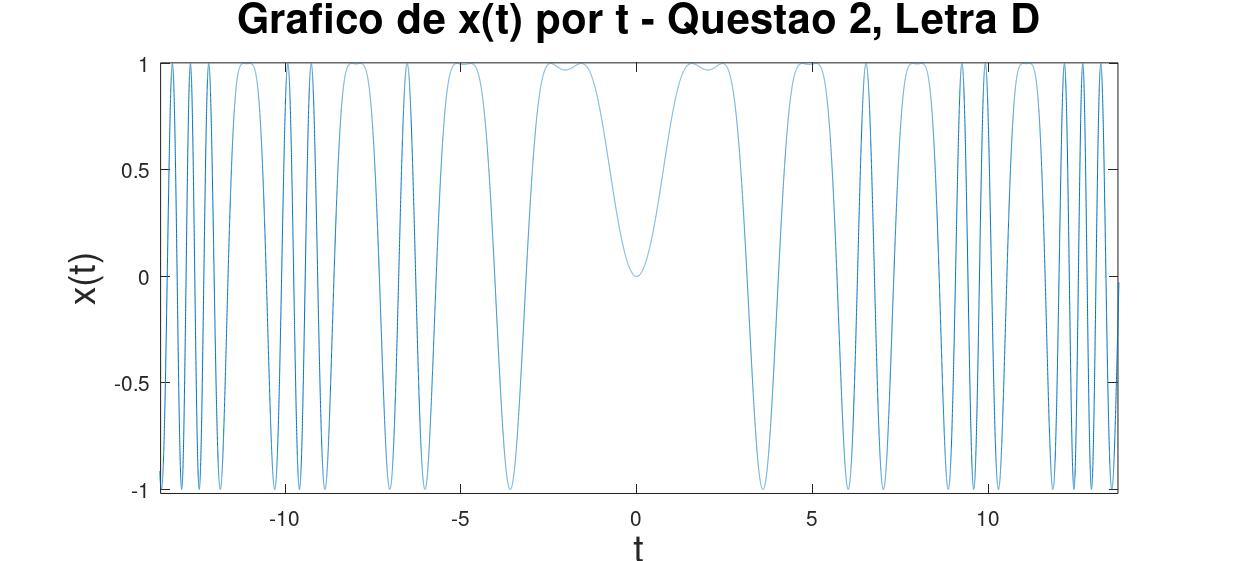
\includegraphics[scale=0.3]{plot2d}
    \centering
\end{figure}

\vspace{\baselineskip}

Do gráfico, nota-se que este sinal não é periódico. As distâncias entre as cristas e entre os vales não é fixa ao longo do gráfico.

\vspace{\baselineskip}

3.) Um sinal periódico com período fundamental $T_{0} = 4 $ é descrito por \textbf{G2}: $x(t) = 1 - e^{|t|}$ para $-T_{0}/2 \leq t < T_{0} / 2$
(a) Esboce o seu gráfico;
(b) calcule analiticamente sua potência total $P$;
(c) calcule $X_{0}$ usando $k = 0$ na fórmula geral de $X_{k}$;
(d) calcule analiticamente os coeficientes $X_{k}$ e verifique se a expressão obtida leva a $X_{0}$ sem indeterminações;
(e) esboce os espectros de módulo e fase;
(f) para $k = 0, 1, 2\;e\;3$, calcule a potência acumulada $P_{k}^{a}$ contida nos harmônicos de $0\;a\;k$;
(g) para $k = 0, 1, 2\;e\;3$, calcule a potência relativa $P_{k}^{a}/P$;
(h) quantos harmônicos são necessários para uma aproximação reter $90.00\%$ da potência?

\vspace{\baselineskip}

(b) Podemos, inicialmente, calcular a energia do sinal no período $[-2\;2]$ com $T_{0} = 4$ e $\omega_{0} = \frac{2 \pi}{T_{0}} = \frac{\pi}{2}$.\\
$E = \int_{-2}^{2} \mid x(t) \mid ^{2}\,dt = \int_{-2}^{0} \mid 1 - e^{\mid t\mid} \mid^{2}\,dt + \int_{0}^{2} \mid 1 - e^{\mid t\mid} \mid^{2}\,dt$

\[E = \int_{-2}^{0} (1 - 2e^{\mid t \mid} + e^{2\mid t \mid})\,dt + \int_{0}^{2} (1 - 2e^{\mid t \mid} + e^{2\mid t \mid})\,dt =\]
\[E = (t - 2e^{\mid t \mid} + \frac{1}{2}e^{2 \mid t \mid}) \mid_{-2}^{0} + (t - 2e^{\mid t \mid} + \frac{1}{2}e^{2 \mid t \mid}) \mid_{0}^{2} = \]
\[E = (0 -2 + \frac{1}{2} - (-2 - 2e^{2} + \frac{1}{2}e^{4})) + (2 - 2e^{2} + \frac{1}{2}e^{4}) - (0 -2 + \frac{1}{2}) = 4\]
\[E = 4\]
A potência, portanto, será calculada como a energia dividida pelo período de tempo calculado: $P = \frac{E}{4} = 1$.

\vspace{\baselineskip}

(c) A fórmula geral de $X_{k}$ é dada por:
\[X_{k} = \frac{1}{T_{0}} \int_{T_{0}} x(t)\,e^{-jkw_{0}t}\,dt\]
Para o nosso caso:
\[X_{0} = \frac{1}{4} \biggl[\int_{-2}^{0} (1 - e^{-t})\,dt + \int_{0}^{2} (1 - e^{t})\,dt\biggr]\]
\[X_{0} = \frac{1}{4} \biggl[\bigl(t + e^{-t}\bigr)_{-2}^{0} + \bigl(t - e^{t}\bigr)_{0}^{2}\biggr]\]
\[X_{0} = \frac{1}{4} \biggl[\bigl(0 + 1\bigr) - \bigl(-2 + e^{2}\bigr) + \bigl(2 - e^{2}\bigr) - \bigl(0 - 1\bigr)\biggr]\]
\[X_{0} = \frac{3 - e^{2}}{2}\]
O termo DC, vale $\frac{3 - e^{2}}{2}$.

\vspace{\baselineskip}

(d) Já temos a fórmula geral de $X_{k}$ acima descrita. Assim, para o caso geral, temos:
\[X_{k} = \frac{1}{4}\biggl[\int_{-2}^{2} (1 - e^{\mid t \mid})\,e^{-jk\frac{\pi}{2}t}\,dt\biggr]\]
\[X_{k} = \frac{1}{4}\biggl[\int_{-2}^{0} (1 - e^{-t})\,e^{-jk\frac{\pi}{2}t}\,dt + \int_{-2}^{0} (1 - e^{t})\,e^{-jk\frac{\pi}{2}t}\,dt\biggr]\]

\vspace{\baselineskip}

Para facilitar as contas, e a visualização, chamaremos a constante $jk\frac{\pi}{2}$ de $c$.

\vspace{\baselineskip}

\[X_{k} = \frac{1}{4} \biggl[\int_{-2}^{0} (1 - e^{-t})\,e^{-ct}\,dt + \int_{0}^{2} (1 - e^{t})\,e^{-ct}\,dt\biggr]\]
\[X_{k} = \frac{1}{4} \biggl[\int_{-2}^{0} (e^{-ct} - e^{-t(c + 1)})\,dt + \int_{0}^{2} (e^{-ct} - e^{t(1 - c)}\,dt)\biggr]\]
\[4X_{k} = \Biggl(\frac{-e^{-ct}}{c} - \biggl(\frac{-e^{-t(c+1)}}{c + 1}\biggr)\Biggr)_{-2}^{2} + \Biggl(\frac{-e^{-ct}}{c} - \frac{e^{t(1 - c)}}{1 - c}\Biggr)_{0}^{2}\]
\[4X_{k} = \Biggl(-\frac{1}{c} + \frac{1}{c + 1} + \frac{e^{2c}}{c} - \frac{e^{2(c + 1)}}{c + 1}\Biggr) + \Biggl(- \frac{e^{-2c}}{c} - \frac{e^{2(1 - c)}}{1 - c} + \frac{1}{c} + \frac{1}{1-c}\Biggr)\]
\[4X_{k} = \Biggl(\frac{1}{c + 1} + \frac{1}{1-c} + \frac{e^{2c}}{c} - \frac{e^{2(c + 1)}}{c + 1} - \frac{e^{-2c}}{c} - \frac{e^{2(1 - c)}}{1 - c} \Biggr)\]

Substituindo $c$ pela constante $jk\frac{\pi}{2}$, chegamos à expressão final:

\[X_{k} = \frac{2}{k^2\pi^2 + 4} - \frac{2e^2}{k^2\pi^2 + 4}cos(k\pi) + sinc(k)\]

Que pode ser simplificada para:

\[X_{k} = \frac{2}{k^2\pi^2 + 4} - \frac{2e^2}{k^2\pi^2 + 4}(-1)^{k} + sinc(k)\]

Perceba, então, que não existe indeterminações na expressão $X_{k}$, na qual podemos, inclusive, calcular para $k = 0$.
\[X_{0} = \frac{2}{4} - \frac{2e^2}{4}(-1)^{0} + sinc(0)\]
\[X_{0} = \frac{1}{2} - \frac{e^2}{2} + 1\]
\[X_{0} = \frac{3 - e^2}{2}\]

Que foi a expressão inicialmente obtida.

\vspace{\baselineskip}

4.) O grupo $i$ trabalhará com o sinal periódico $x(t)$ usado pelo grupo $i + 1$ na questão 1 (ao grupo 7: sinal 1). As aproximações numéricas para Octave/MatLab vistas, podem e devem ser utilizadas.
(a) Traçar gráfico;
(b) encontrar potência total $P$;
(c) calcular os $X_{k}$ para $k \in [-10\;10]$;
(d) traçar os espectos de magnitude, fase e potência;
(e) estimar quantos harmônicos são necessários para reter $90.00\%$ da potência;
(f) calcular os coeficientes $a_{k}\;e\;b_{k}$ correspondentes;
(g) traçar, num mesmo gráfico, $x(t)$ e as aproximações.

Sinal a ser estudado: {\textbf G3}: $x(t) = -t - 5, -2, -t^3 + 3t, 2, -t + 5$ para o intervalo $I_{1} = [-5\;-3], I_{2} = [-3\;-1], I_{3} = [-1\;1], I_{4} = [1\;3], I_{5} = [3\;5]$.

\newpage

(a) Traçando o gráfico do sinal periódico:

\begin{figure}[!ht]
    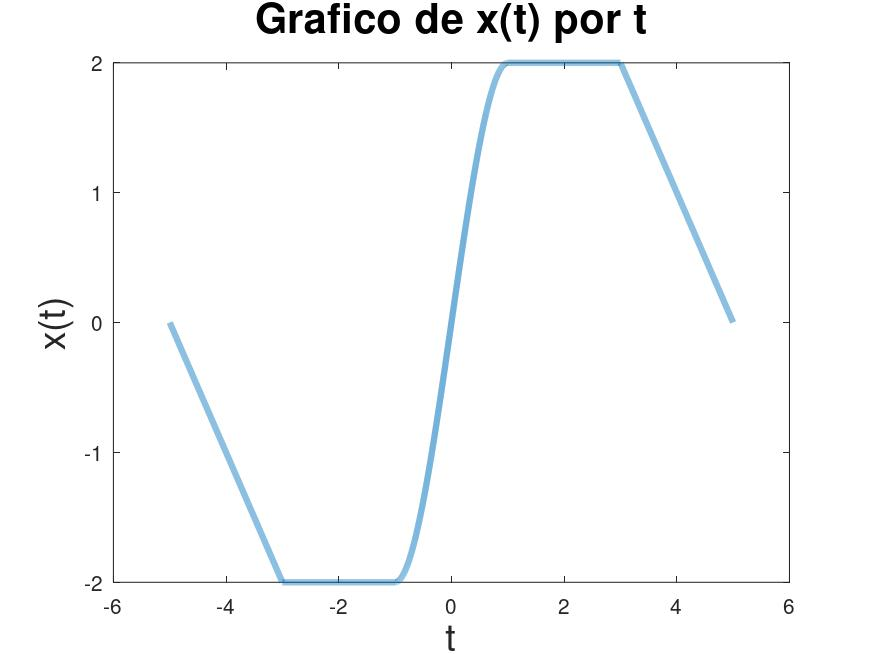
\includegraphics[scale=0.3]{plot4a}
    \centering
\end{figure}

\vspace{\baselineskip}

(b) Encontrando a potência total $P$ com a aproximação da fórmula $P_{[-5\;5]} = \frac{1}{5 - (-5)} \int_{-5}^{5} |x(t)|^2 dt $:

\vspace{\baselineskip}

Potência total $(P)$ = 2.5219

\vspace{\baselineskip}

(c) Calculando os $X_{k}$ para $k \in [-10\;10]$:

\begin{align*}
    X_{-10} &=  3.6250 \times 10^{-17} - 4.8377\times 10^{-3}j; & X_{10} &=  3.6250\times 10^{-17} + 4.8377\times 10^{-3}j.\\
    X_{-9} &=  1.3859\times 10^{-18} - 1.2007\times 10^{-2}j;   & X_{9} &=  1.3859\times 10^{-18} + 1.2007\times 10^{-2}j;\\
    X_{-8} &=  1.5344\times 10^{-17} - 5.4810\times 10^{-5}j;   & X_{8} &=  1.5344\times 10^{-17} + 5.4810\times 10^{-5}j;\\
    X_{-7} &= -1.1824\times 10^{-18} + 7.3857\times 10^{-3}j;   & X_{7} &= -1.1824\times 10^{-18} - 7.3857\times 10^{-3}j;\\
    X_{-6} &= -3.0899\times 10^{-17} + 1.2438\times 10^{-3}j;   & X_{6} &= -3.0899\times 10^{-17} - 1.2438\times 10^{-3}j;\\
    X_{-5} &=  1.6911\times 10^{-17} + 3.8702\times 10^{-2}j;   & X_{5} &=  1.6911\times 10^{-17} - 3.8702\times 10^{-2}j;\\
    X_{-4} &=  3.1526\times 10^{-17} + 1.0894\times 10^{-1}j;   & X_{4} &=  3.1526\times 10^{-17} - 1.0894\times 10^{-1}j;\\
    X_{-3} &= -6.7537\times 10^{-18} + 1.1269\times 10^{-1}j;   & X_{3} &= -6.7537\times 10^{-18} - 1.1269\times 10^{-1}j;\\
    X_{-2} &=  1.4539\times 10^{-17} + 1.9635\times 10^{-1}j;   & X_{2} &=  1.4539\times 10^{-17} - 1.9635\times 10^{-1}j;\\
    X_{-1} &=  1.4886\times 10^{-17} + 1.0936j;                  & X_{1} &=  1.4886\times 10^{-17} - 1.0936j;\\
    X_{o} &= 6.3307\times 10^{-17}; &
\end{align*}

\newpage

(d) Traçando os espectros de magnitude, fase e potência:

\vspace{\baselineskip}

\begin{figure}[h!]
    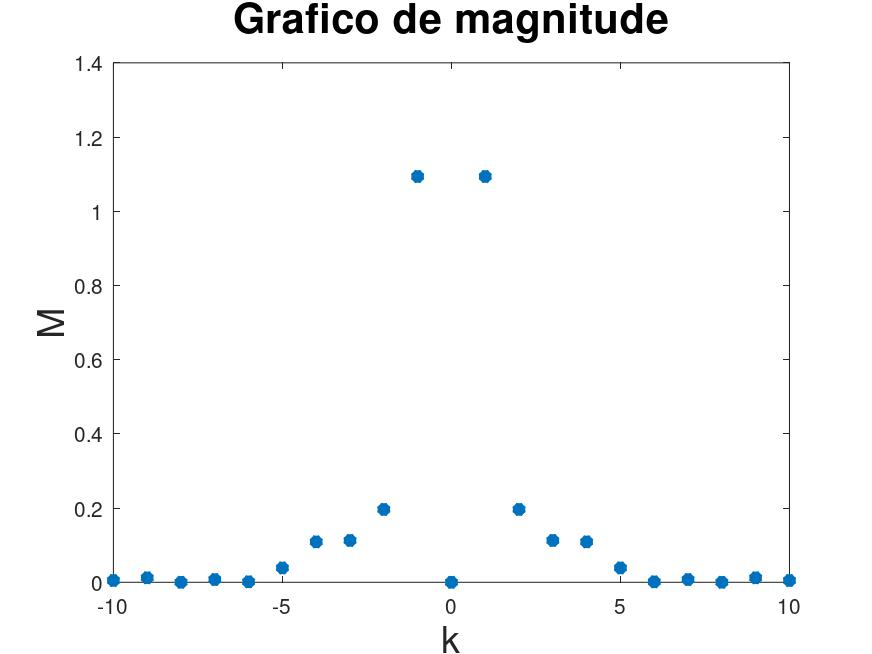
\includegraphics[scale=0.3]{plot4dm}
    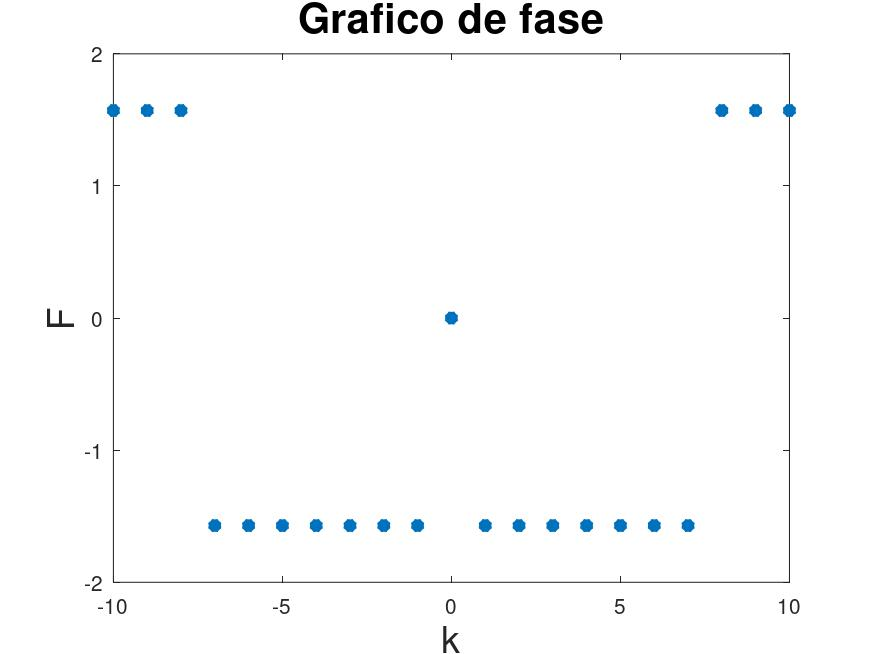
\includegraphics[scale=0.3]{plot4df}
    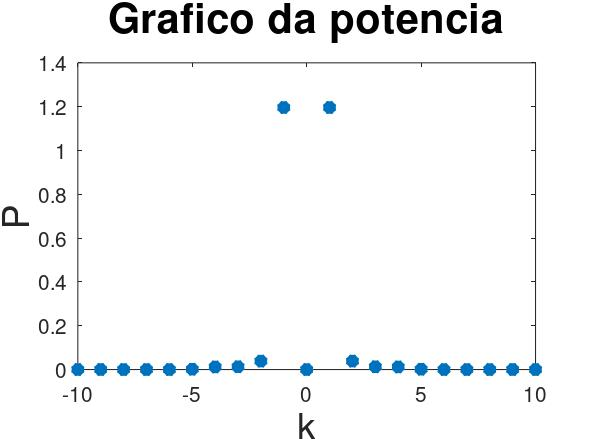
\includegraphics[scale=0.43]{plot4dp}
    \centering
\end{figure}

(e) Calculando $a_{k}$ e $b_{k}$ a partir dos coeficientes $X_{k}$, teremos:

\begin{align*}
    a_{0} &= 6.3307\times 10^{-17}   &   b_{0} &= 0\\
    a_{1} &= 2.9772\times 10^{-17}   &   b_{1} &= 2.1873\\
    a_{2} &= 2.9078\times 10^{-17}   &   b_{2} &= 0.3927\\
    a_{3} &= -1.3507\times 10^{-17}  &   b_{3} &= 0.2254\\
    a_{4} &= 6.3052\times 10^{-17}   &   b_{4} &= 0.2179\\
    a_{5} &= 3.3822\times 10^{-17}   &   b_{5} &= 0.077404\\
    a_{6} &= -6.1798\times 10^{-17}  &   b_{6} &= 2.4876\times 10^{-3}\\
    a_{7} &= -2.3649\times 10^{-18}  &   b_{7} &= 0.014771\\
    a_{8} &= 3.0689\times 10^{-17}   &   b_{8} &= -1.0962\times 10^{-4}\\
    a_{9} &= 2.7717\times 10^{-18}   &   b_{9} &= -0.024014\\
    a_{10} &= 7.2500\times 10^{-17}  &   b_{10} &= -9.6755\times 10^{-3}
\end{align*}

(e) Estimando quantos harmônicos são necessários para reter $90.00\%$ da potência:

\vspace{\baselineskip}

Até o primeiro harmônico que consegue reter $94,85\% $

\vspace{\baselineskip}

5.) Na escala de tempo {\tt t=0:1/2000:5}, considere um sinal de áudio simples $x_{b}(t) = sen(2 \pi f_{0}t)$ ou $x_{b}(t) = cos(2 \pi f_{0}t)$ com frequência \textbf{G2:} $f_{0} = 132Hz$. Ouça este som usando o comando {\tt sound(xb)} no Octave; o resultado é, provavelmente, desagradável pois se trata de uma frequência pura e a sensação é seca, metálica. Para melhorar o \textbf{timbre} do som é preciso colocar mais harmônicos. Crie, na mesma escala de tempo, com a mesma frequência fundamental $f_{0}$, com parâmetros a seu critério e usando até o harmônico $k = 6\;(6f_{0}Hz)$ os sinais a seguir. Ouça cada um deles e compare a qualidade do timbre.\\
(a) Uma onda quadrada $x_{q}(t)$;
(b) uma onda triangular $x_{t}(t)$;
(c) um seno semi-retificado sem o nível DC $x_{s}(t)$;
(d) Opcional: adicionando senos e co-senos harmônicos a seu critério, imagine-se projetando um sintetizador de som e crie um sinal periódico $x(t)$ com frequência fundamental $f_{0}$ e um timbre agradável.


\end{document}
